\documentclass[12pt,aspectratio=169]{beamer}
\usetheme{default}
\usecolortheme{dolphin}
\usefonttheme{structurebold}
\setbeamertemplate{footline}[frame number]

\title{ShellScript 01}
\author{@aoirint}
\date{2020/04/16}
%\institute{}

\begin{document}

% 01
\frame{\maketitle}

% 02
\begin{frame}{テキスト}

  \begin{minipage}{0.58\textwidth}
    \begin{itemize}
      \item 新しいシェルプログラミングの教科書
      \begin{itemize}
        \item 著・三宅英明
        \item 刊・SB Creative
      \end{itemize}
    \end{itemize}
  \end{minipage}
  \hfill
  \begin{minipage}{0.38\textwidth}
    \vspace{-4\baselineskip}
    \begin{center}
      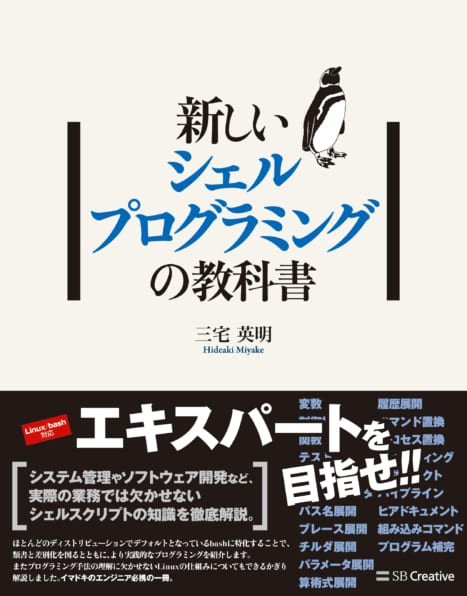
\includegraphics[width=5cm,bb=0 0 467 596]{./images/shellbook.jpg}
    \end{center}
  \end{minipage}

  \begin{itemize}
    \item 書影
    \begin{itemize}
      \item { \small \url{https://www.sbcr.jp/product/4797393101/} }
    \end{itemize}
  \end{itemize}

\end{frame}


\begin{frame}{シェル:GUI(Graphical User Interface)}

  \begin{minipage}{0.45\textwidth}
    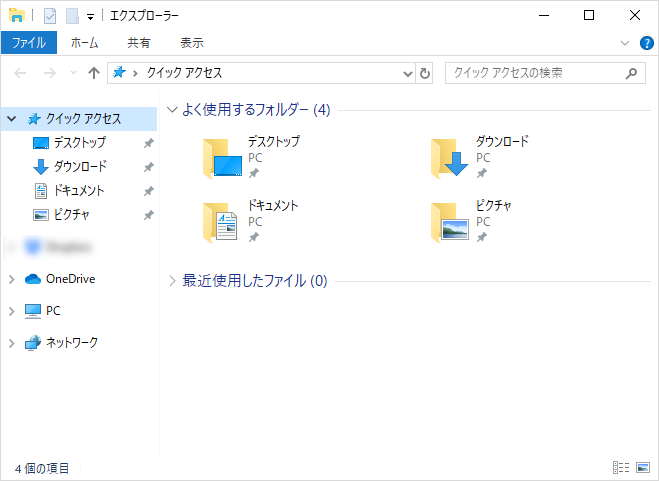
\includegraphics[width=6cm,bb=0 0 659 481]{./images/explorer.png}
    Explorer(Windows)
  \end{minipage}
  \hfill
  \begin{minipage}{0.45\textwidth}
    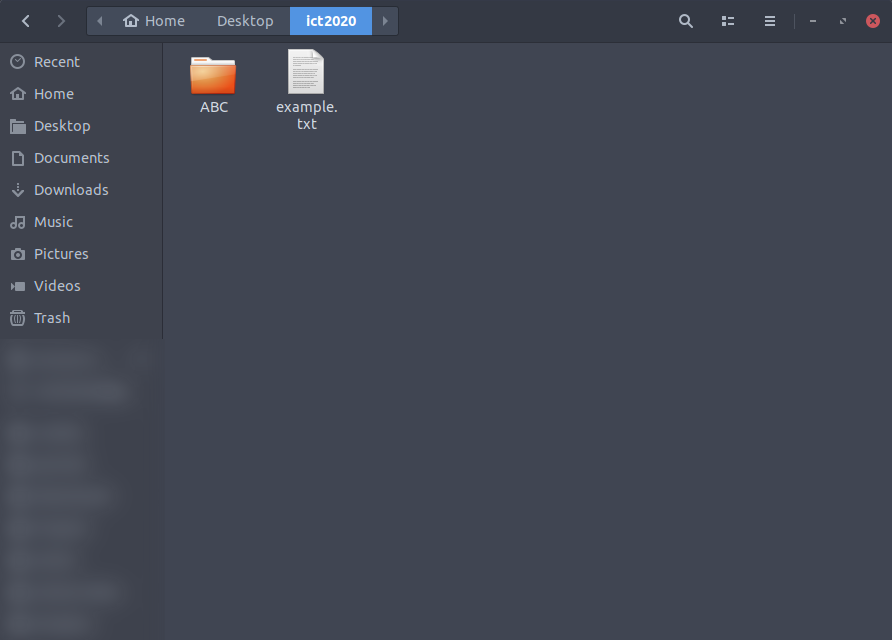
\includegraphics[width=6cm,bb=0 0 892 640]{./images/nautilus.png}
    Nautilus(Ubuntu, Gnome)
  \end{minipage}

\end{frame}


\begin{frame}{シェル:CLI(Command Line Interface)}

  \begin{minipage}{0.3\textwidth}
    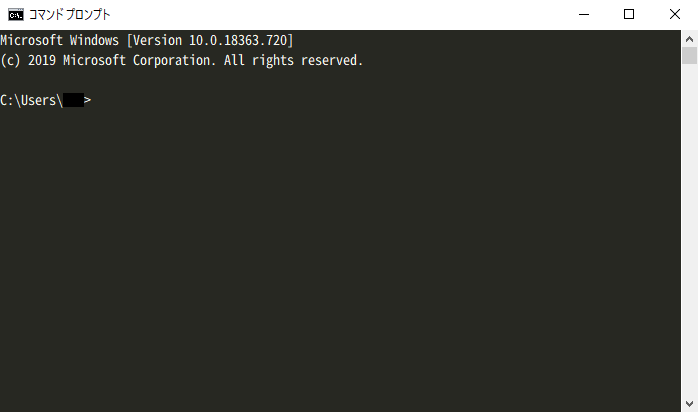
\includegraphics[width=1.2\linewidth,bb=0 0 698 412]{./images/cmd.png}
    コマンドプロンプト(cmd.exe; Windows)

    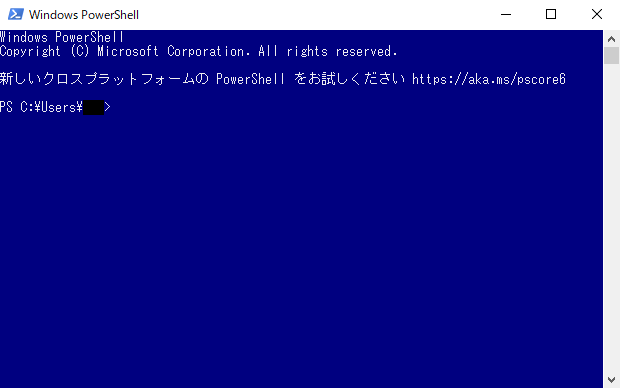
\includegraphics[width=1.2\linewidth,bb=0 0 620 388]{./images/powershell.png}
    PowerShell(Windows)
  \end{minipage}
  \hfill
  \begin{minipage}{0.3\textwidth}
    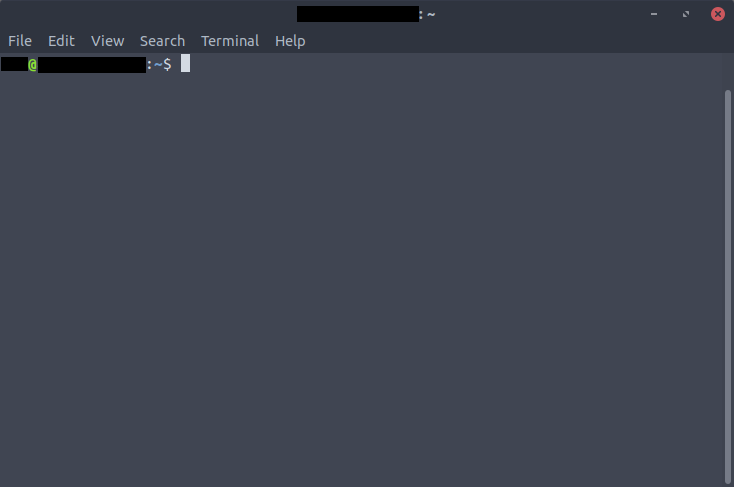
\includegraphics[width=\linewidth,bb=0 0 734 487]{./images/ubuntu-gnome.png}
    \begin{flushleft} \small bash(Ubuntu, Gnome Terminal) \end{flushleft}
    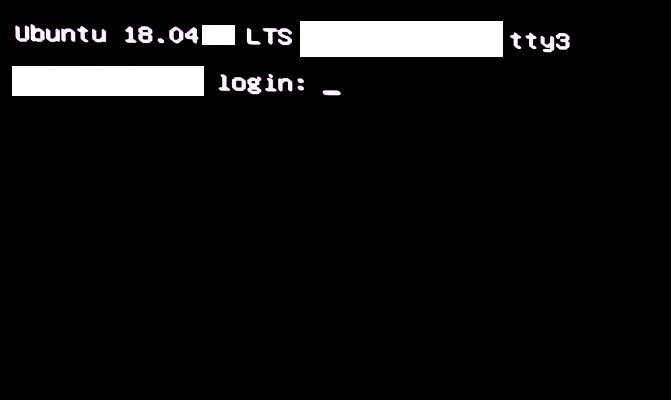
\includegraphics[width=\linewidth,bb=0 0 1262 721]{./images/ubuntu-cli.jpg}
    bash(Ubuntu, CLI)
  \end{minipage}
  \hfill
  \begin{minipage}{0.3\textwidth}
    \vspace{-5\baselineskip}
    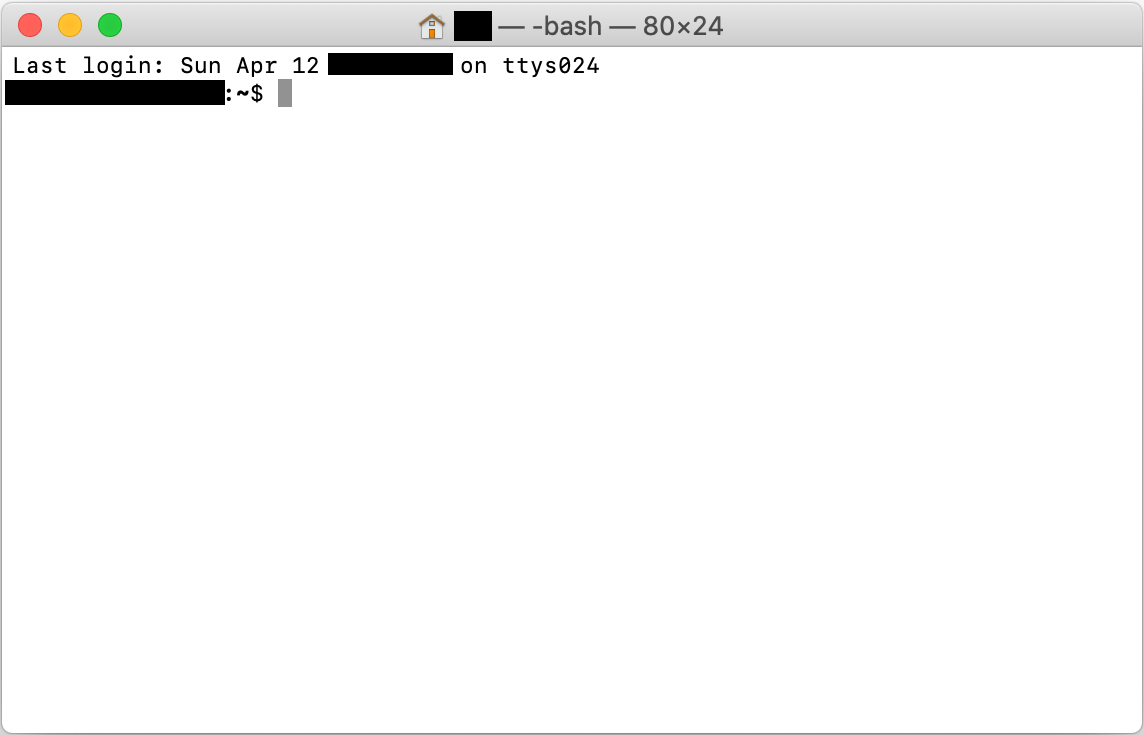
\includegraphics[width=2.0\linewidth,bb=0 0 1144 735]{./images/mac-basic.png}
    bash(macOS, Terminal)
  \end{minipage}

\end{frame}


\begin{frame}{シェルはどこに位置するか}
  \centering
  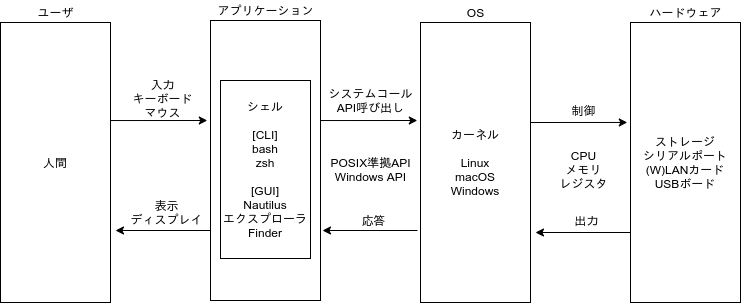
\includegraphics[width=12cm,bb=0 0 741 281]{./images/shell.png}

\end{frame}


\begin{frame}{OSとカーネル}
  \begin{itemize}
    \item カーネル(Kernel)
      \begin{itemize}
        \item OSの核となる(中心的な)機能の実装
          \begin{itemize}
            \item ファイルシステム、ネットワーク、入出力、プロセス管理など
          \end{itemize}
        \item 例:Linuxカーネル、macOSカーネル(XNU)、Windowsカーネル
        \item 余談:Linuxディストリビューションと呼ばれるOSのカーネルはLinuxカーネルをベースにしている
          \begin{itemize}
            \item Debian GNU/Linux、Ubuntu、CentOSなど
          \end{itemize}
      \end{itemize}

      \item OS
        \begin{itemize}
          \item カーネルにハードウェアドライバや標準のソフトウェアなどを追加したパッケージ
          \item 例:Ubuntu、CentOS、macOS、Windows(バージョン略)
        \end{itemize}

      \item 例:C言語のfopen, fprintf, fcloseはファイルシステムに関するカーネルの機能を(最終的に)呼び出す関数(システムコール)
  \end{itemize}

\end{frame}


\begin{frame}{シェルとコマンド 1/2}
  \begin{itemize}
    \item シェル(Shell)
      \begin{itemize}
        \item コマンドによりカーネルの機能を利用するためのアプリケーションの一種
          \begin{itemize}
            \item 例:ファイルの作成、削除、プロセス管理、他のアプリケーションの起動
          \end{itemize}
        \item ユーザに提供されるコマンドベースのカーネルへのインタフェース
          \begin{itemize}
            \item カーネル/核 の 殻/シェル
          \end{itemize}
        \item 例:sh, bash, zsh, csh, コマンドプロンプト(cmd.exe), PowerShellなど
        \item *shという名前のシェルはよく共通のコマンドを持っている
      \end{itemize}
    \item シェルコマンド
      \begin{itemize}
        \item 例:*shのコマンドls、cmd.exeのコマンドdir、PowerShellのコマンドGet-ChildItemはディレクトリ中のファイルリストを表示する
      \end{itemize}
  \end{itemize}

\end{frame}


\begin{frame}{シェルとコマンド 2/2}
  \begin{itemize}
    \item シェルコマンド
      \begin{itemize}
        \item 例:*shのコマンドls、cmd.exeのコマンドdir、PowerShellのコマンドGet-ChildItemはディレクトリ中のファイルリストを表示する
      \end{itemize}
  \end{itemize}

  \centering {
    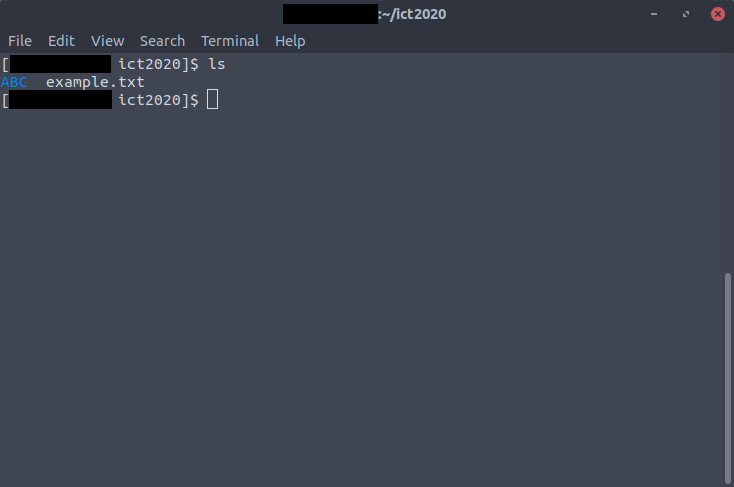
\includegraphics[width=6cm,bb=0 0 659 481]{./images/ls.png}
  }

\end{frame}


\begin{frame}{Explorerもシェル}

  \begin{minipage}{0.45\textwidth}
    \begin{itemize}
      \item Explorer(Windows)もシェル
        \begin{itemize}
          \item GUIなのにコマンド?
        \end{itemize}
      \item 例:コンテキストメニュー(右クリックメニュー)の動作
        \begin{itemize}
          \item レジストリ中にテキスト形式のコマンドで定義されている
          \item { \tiny 余談 }
            \begin{itemize}
              \item { \tiny レジストリを編集すれば自分でメニューを追加することもできる(間違ったところをいじらないように注意は必要) }
              \item { \tiny u\_atomhere, u\_conemuhereは自分で追加した項目 }
            \end{itemize}
        \end{itemize}
    \end{itemize}

  \end{minipage}
  \hfill
  \begin{minipage}{0.45\textwidth}
    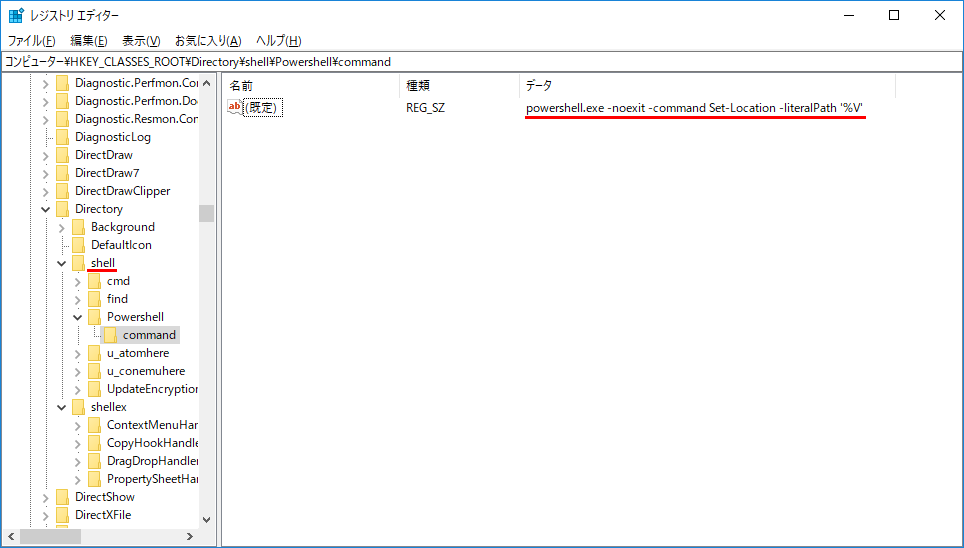
\includegraphics[width=6cm,bb=0 0 659 481]{./images/regedit.png}
    { \tiny Windowsのレジストリ(フォルダをShift+右クリックしたときの「PowerShellで開く」コマンド) }
  \end{minipage}

\end{frame}


\begin{frame}{ログインシェル}
  \begin{itemize}
    \item テキストではbashを題材にしているので、ここからはUNIX, bashを前提とする

    \item ログインシェル
      \begin{itemize}
        \item デフォルトで使われるシェルのこと
        \item ログインシェルの指定はユーザ情報を保管するファイル/etc/passwdなどに書かれている
      \end{itemize}

  \end{itemize}

\end{frame}
\begin{frame}{シェルとプロセス 1/2}
  \begin{itemize}
    \item プロセスの親子関係
      \begin{itemize}
        \item シェル上でコマンドを実行したとき、シェルのプロセスに対する子プロセスが生成される
      \end{itemize}
    \item 子プロセス
      \begin{itemize}
        \item 親となるプロセスのメモリ内容(アドレス空間)をコピーして作られる
        \item メモリがコピーされているため、親プロセスのシェル上の環境変数などを引き継ぐ
        \item プログラムを呼び出すコマンドが実行されると、forkシステムコールにより子プロセスが生成されたあと、exec系システムコールによりプログラムが子プロセスのアドレス空間(メモリ領域)に読み出される
      \end{itemize}

  \end{itemize}

\end{frame}


\begin{frame}{シェルとプロセス 2/2}
  \begin{itemize}
    \item psコマンド
      \begin{itemize}
        \item プロセスリストを表示するコマンド
        \item ps fはプロセスの親子関係をグラフィカルに表示する
      \end{itemize}
  \end{itemize}

  \centering {
    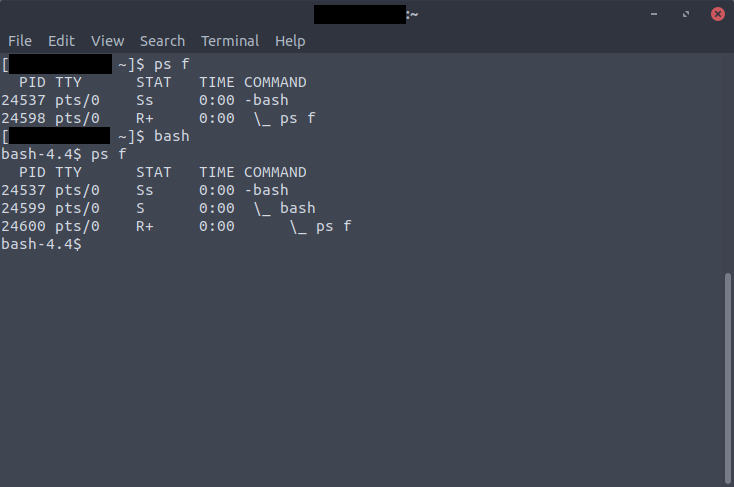
\includegraphics[width=6cm,bb=0 0 734 487]{./images/child-process.png}
  }

  \begin{itemize}
    \item 親プロセスはbash(ID 24537)、プログラム/usr/bin/bashを呼び出して子プロセスbash(ID 24599)が生成されている
      \begin{itemize}
        \item また、psコマンド自体も子プロセスとして実行されている
      \end{itemize}
  \end{itemize}

\end{frame}


\begin{frame}{シェルスクリプトとは}
  \begin{itemize}
    \item シェルのコマンドを列挙したテキストファイル
    \item ファイルをシェルプログラムに与えることで実行する
    \item 複数のコマンドや複雑なコマンドをいちいち入力する必要がなくなる
      \begin{itemize}
        \item 複数のコマンド
          \begin{itemize}
            \item コマンドを組み合わせた定型処理
          \end{itemize}
        \item 複雑なコマンド
          \begin{itemize}
            \item たくさんのオプションを指定するプログラム
            \item 例:動画像・音声処理プログラムのffmpegなど
          \end{itemize}
        \item if, forなどの制御構造を含むプログラム
        \item 起動時・ログイン時の初期化プログラム
      \end{itemize}
  \end{itemize}

\end{frame}


\begin{frame}{シェルスクリプトを実行する}
  \begin{itemize}
    \item command.shファイルを作成(echoは文字列を出力するコマンド) \\
      \texttt {
        echo "Hello Shell Script!"
      }
    \item \texttt{bash command.sh} で実行
  \end{itemize}

  \centering {
    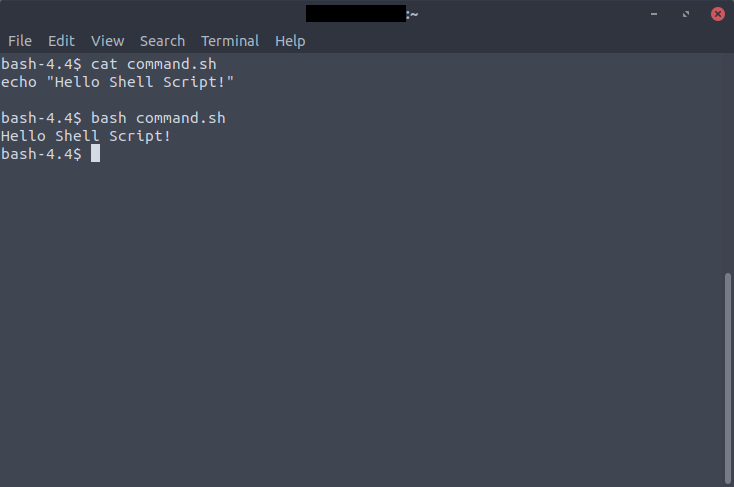
\includegraphics[width=6cm,bb=0 0 734 487]{./images/exec-sh.png}
  }

\end{frame}


\begin{frame}{shebang}
  \begin{itemize}
    \item command.shの1行目に以下を追記する \\
      \texttt {
        !\#/bin/bash
      }
      \begin{itemize}
        \item これはshebangという記法(/bin は /usr/bin へのシンボリックリンク)
        \item ファイルの実行時にファイルパスを渡すプログラムを記述する(シェルでなくてもよい; ex.CGIスクリプト)
      \end{itemize}
    \item command.shに実行権限を付与する \\
      \texttt {
        chmod +x command.sh
      }
    \item \texttt{./command.sh} で実行
      \begin{itemize}
        \item \texttt{command.sh}を\texttt{command}にリネームすると\texttt{./command}で実行できる
      \end{itemize}

  \end{itemize}

  \centering {
    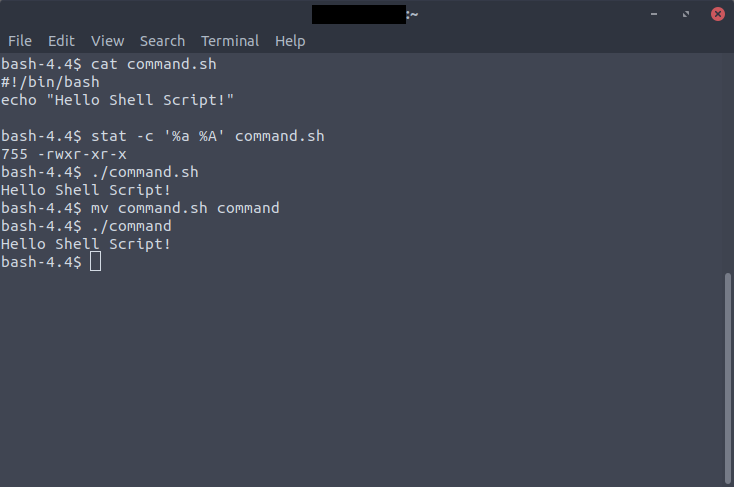
\includegraphics[width=6cm,bb=0 0 734 487]{./images/exec-sh2.png}
  }

\end{frame}


\begin{frame}{シェルスクリプトの記法 1/2}
  \begin{itemize}
    \item 改行
      \begin{itemize}
        \item コマンドとコマンドの区切りは改行で表される
        \item コマンドの途中で改行するときはバックスラッシュ( $\backslash$ )を入れる
          \begin{itemize}
            \item 改行は空白扱いにはならないので注意
            \item ×:\texttt{echo$\backslash$[改行]Hello}
            \item ◯:\texttt{echo $\backslash$[改行]Hello}
            \item ◯:\texttt{ec$\backslash$[改行]ho Hello}
          \end{itemize}

        \item 空行(何も書かれていない行)は無視される
      \end{itemize}

  \end{itemize}

\end{frame}


\begin{frame}{シェルスクリプトの記法 2/2}
  \begin{itemize}
    \item コメント
      \begin{itemize}
        \item 実行されないテキストをスクリプト中に埋め込める
        \item 文字\#以降のその行はコメント\\
          \texttt{echo Hello \# shell says Hello }
        \item コメントアウト(コマンドをコメントにして実行されないようにする)\\
          \texttt{\# echo Hello }
      \end{itemize}

  \end{itemize}

\end{frame}


\begin{frame}{カレントディレクトリとパス 1/2}
  \begin{itemize}
    \item pwd(positioning working directory)コマンド\\
      \texttt{pwd}
      \begin{itemize}
        \item カレントディレクトリを出力する(echoのように)
        \item 相対パスの基点となる
          \begin{itemize}
            \item 絶対パスの例:/home/user/command.sh
            \item 相対パスの例:command.sh または ./command.sh, ../example.txt (.はカレントディレクトリ、..は親ディレクトリを意味する)
          \end{itemize}
      \end{itemize}

  \end{itemize}

\end{frame}


\begin{frame}{カレントディレクトリとパス 2/2}
  \begin{itemize}
    \item cd(change directory)コマンド\\
      \texttt{cd MY\_PATH}
      \begin{itemize}
        \item カレントディレクトリを\texttt{MY\_PATH}に変更する
      \end{itemize}

    \item カレントディレクトリ以外のファイルも実行できる/扱える
      \begin{itemize}
        \item カレントディレクトリが異なると 相対パスで指定したファイルを操作するときの操作対象が変わる
      \end{itemize}

  \end{itemize}

\end{frame}


\begin{frame}{文字コード 1/2}
  \begin{itemize}
    \item 文字コード
      \begin{itemize}
        \item 文字をバイナリデータで表す際の符号
        \item ASCIIで定義されている範囲についてはふつうASCII準拠
          \begin{itemize}
            \item ASCII(アスキー):7ビットに英字・アラビア数字・記号・制御文字が割り当てられた有名な文字コード
          \end{itemize}
        \item Unicode(ユニコード)
          \begin{itemize}
            \item 多言語や絵文字に対応した文字コード
            \item BOMなし UTF-8(主流)
            \item BOMあり UTF-8(Windows メモ帳でいうUTF-8はこれ)
            \item UTF-16など
          \end{itemize}
        \item Shift\_JIS
          \begin{itemize}
            \item 古い日本語文字コード
          \end{itemize}
        \item cp932(Shift\_JISのWindows環境での方言、ANSIとも)
          \begin{itemize}
            \item 文字コードの自動認識に失敗してよく文字化けする
          \end{itemize}
        \item など
      \end{itemize}

  \end{itemize}

\end{frame}


\begin{frame}{文字コード 2/2}
  \begin{itemize}
    \item BOM(Byte Order Mark)
      \begin{itemize}
        \item エンディアンや文字コードの種類を区別するためにテキストファイルの先頭に置かれるバイナリデータ
          \begin{itemize}
            \item エンディアン:2バイト以上のデータを並べる順番
            \item リトルエンディアン、ビッグエンディアン
          \end{itemize}
        \item これを考慮していない環境ではファイルの先頭が文字化けする
          \begin{itemize}
            \item スクリプトなら実行に失敗する
          \end{itemize}
      \end{itemize}

    \item プログラムを書くのに「メモ帳」(notepad.exe)を使わないほうがいい、と思うのはこのあたりのせい
      \begin{itemize}
        \item インデント関連の機能もない
      \end{itemize}

  \end{itemize}

\end{frame}


\begin{frame}{改行コード}
  \begin{itemize}
    \item 改行コード(主にOS依存)
      \begin{itemize}
        \item ASCIIには2種類の改行に関するコードが定義されている
          \begin{itemize}
            \item CR:Carriage Return (0x0D)
            \item LF:Line Feed (0x0A)
          \end{itemize}
        \item OSによってこれらのコードをどう使って改行を表現するかが異なる(あくまでデフォルト値。エディタで設定できる)
          \begin{itemize}
            \item CR+LF:Windows
            \item CR:古いMac
            \item LF:Unix系OS、現在のMac
          \end{itemize}
        \item Windowsでスクリプトを編集すると改行コードCRが紛れ込む可能性がある
          \begin{itemize}
            \item そのままUnix上に持っていって実行するとCRがコマンドの一部として扱われてエラーになるおそれ
          \end{itemize}

      \end{itemize}

  \end{itemize}

\end{frame}


\begin{frame}{ここまでのまとめ}

  \begin{itemize}
    \item シェル
      \begin{itemize}
        \item OSの機能にコマンドベースでアクセスするインタフェース
        \item グラフィカルシェル
        \item コマンドラインシェル
      \end{itemize}
    \item シェルスクリプト
      \begin{itemize}
        \item シェルコマンドをテキストファイルに列挙したもの
        \item シェルのプログラムにファイルパスを渡して実行する
        \item shebangをスクリプトの先頭に書いて実行することもできる
      \end{itemize}
    \item 文字コード・改行コード
      \begin{itemize}
        \item OSをまたぐときは特に注意する
        \item ちゃんとしたエディタを使うのがよい
      \end{itemize}

  \end{itemize}


\end{frame}


\begin{frame}{変数}
  \begin{itemize}
    \item 変数
      \begin{itemize}
        \item 文字列や数値などの値に名前を付けて格納することができる
        \item 変数名にはアルファベットの大文字、小文字・数字・アンダースコアの組み合わせが使える(ただし先頭に数字は使えない)
        \item 例:my\_var, dir1, \_temp, CONST\_VAR, MyName
      \end{itemize}

  \end{itemize}

\end{frame}


\begin{frame}{変数の作成}
  \begin{itemize}
    \item 変数の作成
      \begin{itemize}
        \item C言語などのように事前に宣言する必要はない
        \item 変数に値を代入することで自動的に変数が作成される
        \item 代入 \\
              \texttt{variable=VALUE}
        \item スペースやタブを含む場合は引用符で囲む \\
              \texttt{variable='My variable'} \\
              \texttt{variable="My variable"}
        \item 特に指定しない場合、変数の値は文字列として扱われる(数値として扱う方法もある)
        \item 空文字列の代入 \\
              \texttt{variable=}
      \end{itemize}

  \end{itemize}

\end{frame}


\begin{frame}{変数の参照}
  \begin{itemize}
    \item 変数の参照
      \begin{itemize}
        \item 変数を作成/代入するときは\$を付けたりする必要はなかった
        \item 変数の値を参照するときには変数名の前に\$を付ける \\
              \texttt{echo \$variable}
        \item 一度も値を設定していない変数を参照してもエラーにならない(空文字列として扱われる) \\
              \texttt{echo \$UNDEFINED\_VARIABLE}
        \item 代入時の左辺に\$を付けるとエラーになるので注意
        \item 変数の値と文字列を結合できる \\
              \texttt{echo ABC \$variable DEF}
        \item 変数名と文字列を区別する場合には変数名を\{\}で囲む \\
              \texttt{echo ABC\$\{variable\}DEF}
      \end{itemize}

  \end{itemize}

\end{frame}


\begin{frame}{環境変数とは}
  \begin{itemize}
    \item 環境変数
      \begin{itemize}
        \item 子プロセス(コマンド)に引き継がれる変数
        \item 通常のシェル変数は子プロセスに引き継がれない
        \item forkシステムコールは親プロセスから子プロセスに環境変数をコピーする
        \item 環境変数はプログラム自体を変更せずに設定を切り替えるためによく使われる
          \begin{itemize}
            \item 仮想化ソフトウェアのDocker上でプログラムを動作させるとき、設定のために特に環境変数が使われることが多い
          \end{itemize}

      \end{itemize}

  \end{itemize}

\end{frame}

\begin{frame}{環境変数の例}
  \begin{itemize}
    \item 環境変数LANG
      \begin{itemize}
        \item 使用する言語を表す環境変数
      \end{itemize}

    \item すでに定義されている環境変数を変更するときは通常の変数と同じように代入するだけでよい
  \end{itemize}

  \centering {
    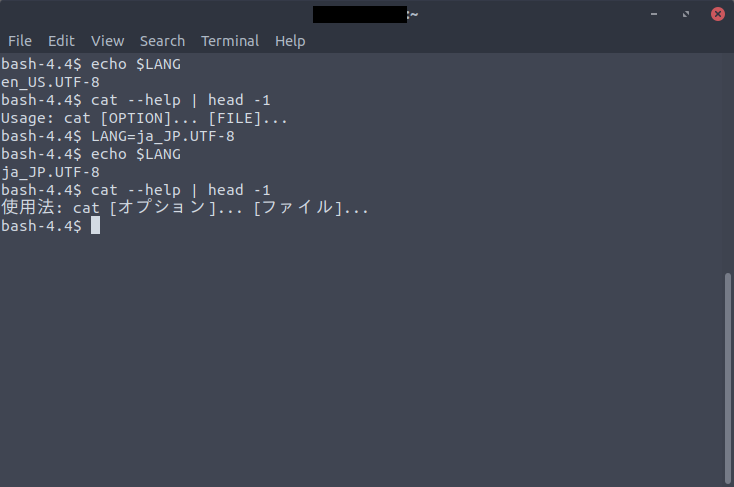
\includegraphics[width=6cm,bb=0 0 734 487]{./images/lang.png}
  }

\end{frame}

\begin{frame}{環境変数の設定}
  \begin{itemize}
    \item exportコマンド
      \begin{itemize}
        \item 変数を環境変数として設定する \\
              \texttt{export variable}
        \item 変数に代入しつつ環境変数として設定する \\
              \texttt{export variable=VALUE}
      \end{itemize}

  \end{itemize}

  \centering {
    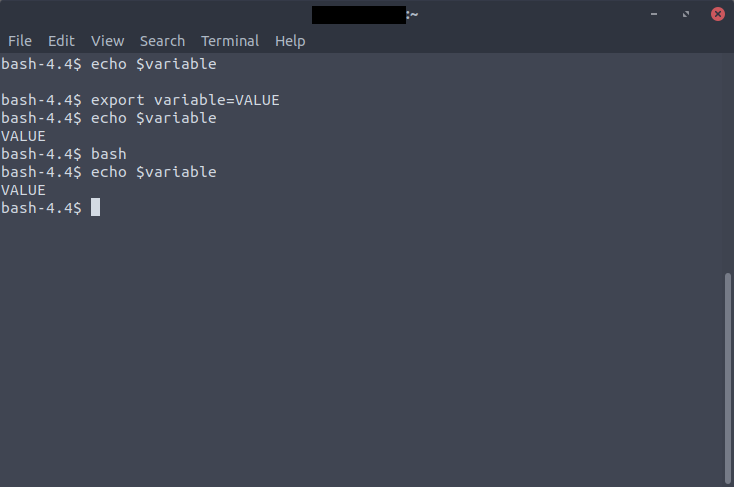
\includegraphics[width=6cm,bb=0 0 734 487]{./images/export.png}
  }

\end{frame}

\begin{frame}{一時的な環境変数の設定}
  \begin{itemize}
    \item コマンドの前に変数への代入を書くことができる \\
          \texttt{variable=VALUE bash}
      \begin{itemize}
        \item このように設定された変数は、子プロセス中でのみ有効な環境変数となる
        \item 親プロセスに復帰したとき、ここで設定した変数の値は反映されない
      \end{itemize}

  \end{itemize}

  \centering {
    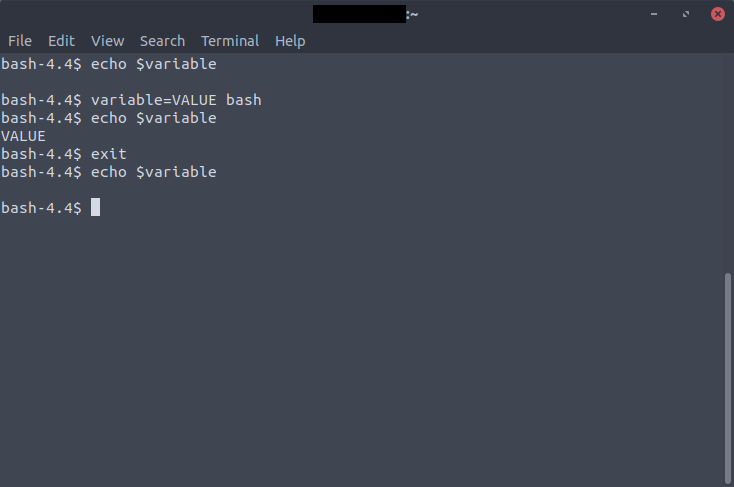
\includegraphics[width=6cm,bb=0 0 734 487]{./images/export2.png}
  }

\end{frame}

\begin{frame}{ここまでのまとめ}
  \begin{itemize}
    \item 変数
      \begin{itemize}
        \item 値に名前を付けて格納できる
        \item 変数への代入 \\
              \texttt{variable=VALUE}
        \item 変数の参照 \\
              \texttt{echo \$variable}
      \end{itemize}
    \item 環境変数
      \begin{itemize}
        \item 子プロセス(コマンド)に引き継がれる変数
        \item 環境変数の設定 \\
              \texttt{export variable=VALUE}
        \item 子プロセス用の環境変数の設定 \\
              \texttt{variable=VALUE command}
      \end{itemize}

  \end{itemize}

\end{frame}

\begin{frame}{参考資料:Beamer}
  \begin{itemize}
    \item \url { https://qiita.com/yt_siden/items/aaac54f6389a8068a4ee }
    \item \url { https://qiita.com/termoshtt/items/756aec542fb4c812a405 }
    \item \url { https://www.opt.mist.i.u-tokyo.ac.jp/~tasuku/beamer.html }
  \end{itemize}

\end{frame}


\begin{frame}{参考資料:OS, カーネル}
  \begin{itemize}
    \item \url { https://ja.wikipedia.org/wiki/Microsoft_Windows }
    \item \texttt {https://ja.wikipedia.org/wiki/Linux\%E3\%83\%87\%E3\%82\%A3 \\ \%E3\%82\%B9\%E3\%83\%88\%E3\%83\%AA\%E3\%83\%93\%E3\%83\%A5\%E3\%83\%BC \\ \%E3\%82\%B7\%E3\%83\%A7\%E3\%83\%B3 }
    \item \url { https://ja.wikipedia.org/wiki/POSIX }
    \item \url { https://ja.wikipedia.org/wiki/Debian }
    \item \url { https://ja.wikipedia.org/wiki/MacOS }
    \item \url { https://ja.wikipedia.org/wiki/XNU }
    \item \url { https://www.atmarkit.co.jp/ait/articles/1112/13/news117.html }
    \item \texttt {https://ja.wikipedia.org/wiki/\%E3\%82\%AA\%E3\%83\%9A \\ \%E3\%83\%AC\%E3\%83\%BC\%E3\%83\%86\%E3\%82\%A3\%E3\%83\%B3\%E3\%82\%B0 \\ \%E3\%82\%B7\%E3\%82\%B9\%E3\%83\%86\%E3\%83\%A0 }
  \end{itemize}

\end{frame}


\begin{frame}{参考資料:プロセス}
  \begin{itemize}
    \item \url { https://ja.wikipedia.org/wiki/Fork }
    \item \url { https://kazmax.zpp.jp/linux_beginner/process_ps.html }
  \end{itemize}

\end{frame}


\begin{frame}{参考資料:スクリプト}
  \begin{itemize}
    \item \texttt {https://docs.microsoft.com/ja-jp/powershell/scripting/\\ samples/working-with-files-and-folders }
    \item \url { https://ja.wikipedia.org/wiki/Pwd }
  \end{itemize}

\end{frame}


\end{document}
